\documentclass[a4paper, 10pt, oneside]{article}

%%%
% https://en.wikibooks.org/wiki/LaTeX/Title_Creation
%%%

\usepackage[utf8]{inputenc}
\usepackage[T1]{fontenc}
\usepackage{lmodern} % Enlève plein de warnings :D et permet le tt gras
\usepackage[frenchb, english]{babel}
\usepackage{geometry}
\usepackage{numprint}

\usepackage{color}
%\usepackage[usenames,dvipsnames,svgnames,table]{xcolor}

\usepackage{amsmath}
\usepackage{amssymb}
\usepackage{mathrsfs}

\usepackage{hyperref}
\hypersetup{
	pdfborder={0 0 0},
	colorlinks=true,
	linkcolor=[rgb]{0,0,0.42},
	citecolor=[rgb]{0.7,0,0.7},
	urlcolor=[rgb]{0,0,0.8}
}
\usepackage{caption}
\usepackage[hyperpageref]{backref}

\usepackage{graphicx}
\usepackage{tikz}

% ----------------------------------------------------------------------------------
% Commandes
% ----------------------------------------------------------------------------------

\newcommand{\lien}[2]{\noindent #1 :\\{\small\url{#2}}}

% ----------------------------------------------------------------------------------
% Main
% ----------------------------------------------------------------------------------
\title{Javascript Project Report\\Robocode}
\author{Reynald \bsc{Barbeaut} AND Timothée \bsc{Guy}}
\date{\\\today}

\begin{document}

% ----------------------------------------------------------------------------------
% Titlepage
% ----------------------------------------------------------------------------------
\begin{titlepage}

	\centering
	
\includegraphics[height=1.5cm]{img/logo_figure.png}
	\hspace{1cm}
	
\includegraphics[height=2cm]{img/logo_ufc.png}
	\hspace{1cm}
	
\includegraphics[height=2cm]{img/logo_ufr_st.png}

	\vspace{3cm}

	{\LARGE Javascript Project Report\par}
	\vspace{2cm}
	\rule{\linewidth}{.8pt}\par
	\vspace{0.8cm}
	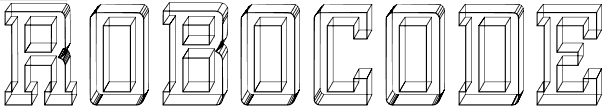
\includegraphics[height=2.5cm]{img/logo_robocode.png}
	\vspace{0.8cm}
	\rule{\linewidth}{.8pt}

	\vspace{2cm}
	{\LARGE Reynald \bsc{Barbeaut} AND Timothée \bsc{Guy}\\}
	\vspace{2cm}
	{\Large L3 CMI Computer-Science\\2017 --- 2018\par}
	\vspace{1cm}
	{\large Teacher: M. Frédéric \bsc{Dadeau}\par}
	{\large FEMTO-ST Institute --- DISC Department\par}

\end{titlepage}

% ----------------------------------------------------------------------------------
% Tables des matières/figures
% ----------------------------------------------------------------------------------
\newpage
\tableofcontents

\newpage
\listoffigures

\newpage
\section{Introduction}
	This report will cover the Javascript project Robocode. Robocode is a two players game where you have to capture flags and bring them back to your base.\\\\
	The application has been made with the following programming languages:
	\begin{itemize}
		\item HTML5
		\item CSS3
		\item Javascript 8
		\item Node.js
	\end{itemize}

\newpage
\section{Features}
	The application is available in two different modes: online multiplayer and local multiplayer. Below, you can see the use case diagram of the application, describing the interactions of the user, that will be described further.
	
	\begin{figure}[h]
		\centering
		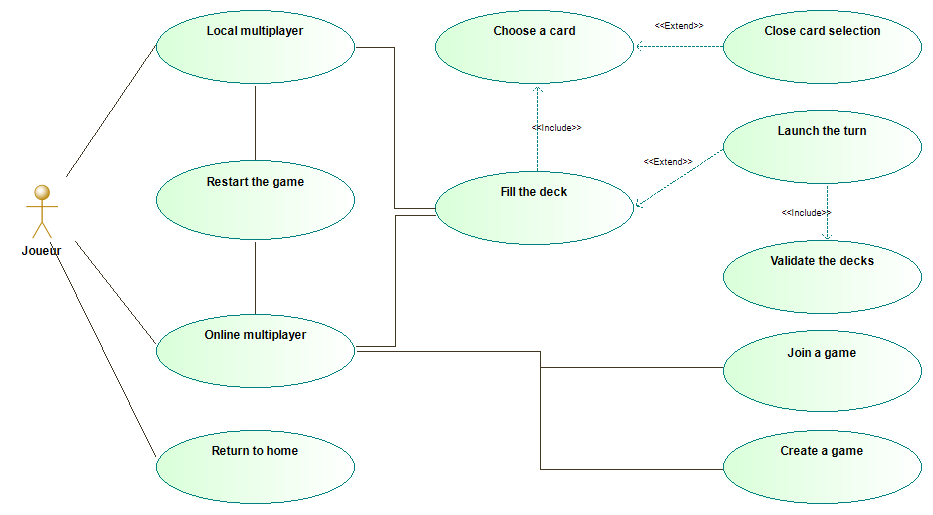
\includegraphics[scale=0.35]{img/use_case.png}
		\caption{Use case diagram}
		\label{fig:UseCase}
	\end{figure}
	
	\subsection{Online/Local multiplayer}
		To use the online multiplayer, the user will have to join the tchat of Robocode and create the game by using the following command in the tchat: \texttt{/invite:username}.
		Then, the other user will have to join the game by using the following command in the tchat: \texttt{/join:username}. When using the local multiplayer mode, the game is launched automatically, because we don't use the tchat to launch it, but a direct HTML link in the homepage of the website.
		
	\subsection{Common features}
		The two modes are distinguished by the way they launch the game, but the core of the game is the same. The game isn't complex, so the user has few numbers of interactions available, he can:
		\begin{itemize}
			\item restart the game: by refreshing the page or clicking on the "restart" button when the game is finished
			\item fill the deck: when the game is launched, the user can fill his deck of cards that will be executed by the robot
			\item choose a card: a window will open where the user can pick a card, in extension, the user can close the card selection window
			\item launch the turn: when either blue and red decks are validated, the player can choose to launch the turn in the local mode, or the server will launch the turn in the online mode
			\item return to home: the user can also choose to return to the homepage of the website
		\end{itemize}

\newpage
\section{Data Models}
	In this project, we used three different class : \texttt{Robot}, \texttt{Flag} and \texttt{Card}. We also used a set of global variables which we aren't going to describe here.

	\begin{figure}[h]
		\centering
		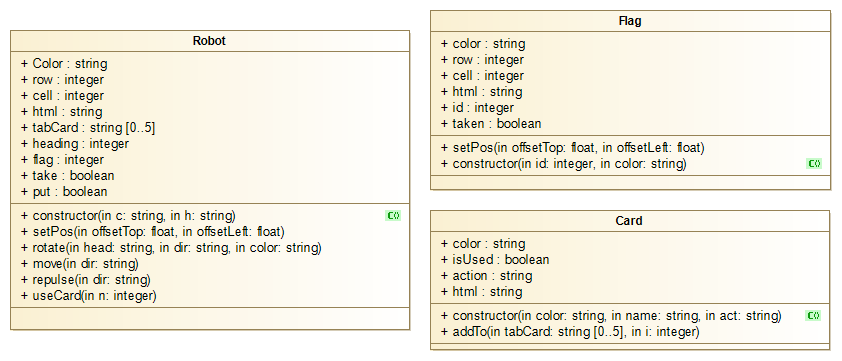
\includegraphics[scale=0.5]{img/class.png}
		\caption{Class diagram}
		\label{fig:Class}
	\end{figure}
	
	\subsection{Robot}
		The class \texttt{Robot} represent a robot. It's used to represent the blue and red robot in the game. It has 9 variables representing different specifications of the robot, and 6 methods detailed below:
			\begin{itemize}
				\item \texttt{constructor}: the constructor of the Class
				\item \texttt{setPos}: sets the position of the robot
				\item \texttt{rotate}: rotates the robot
				\item \texttt{move}: moves the robot in a direction
				\item \texttt{repulse}: repulse another robot
				\item \texttt{useCard}: execute an action of a Card
			\end{itemize}
			
	\subsection{Flag}
		The class \texttt{Flag} represent a flag. It's used to represent all the red and blue flags in the game. It has 6 variables and 2 methods detailed below:
			\begin{itemize}
				\item \texttt{constructor}: the constructor of the Class
				\item \texttt{setPos}: sets the position of the flag
			\end{itemize}
			
	\subsection{Card}
		The class \texttt{Card} represent a card. It's used to represent the different cards in the game. It has 4 variables and 2 methodes detailed below:
			\begin{itemize}
				\item \texttt{constructor}: the constructor of the Class
				\item \texttt{addTo}: adds the Card to a deck
			\end{itemize}
			
\section{Animations}
	There are several animations in the game, one for every movement of the robot (north, south, east, west, eastx2, westx2) and also an animation when the robot is idle or doing an action that doesn't imply moving.
	
	\begin{figure}[h]
		\centering
		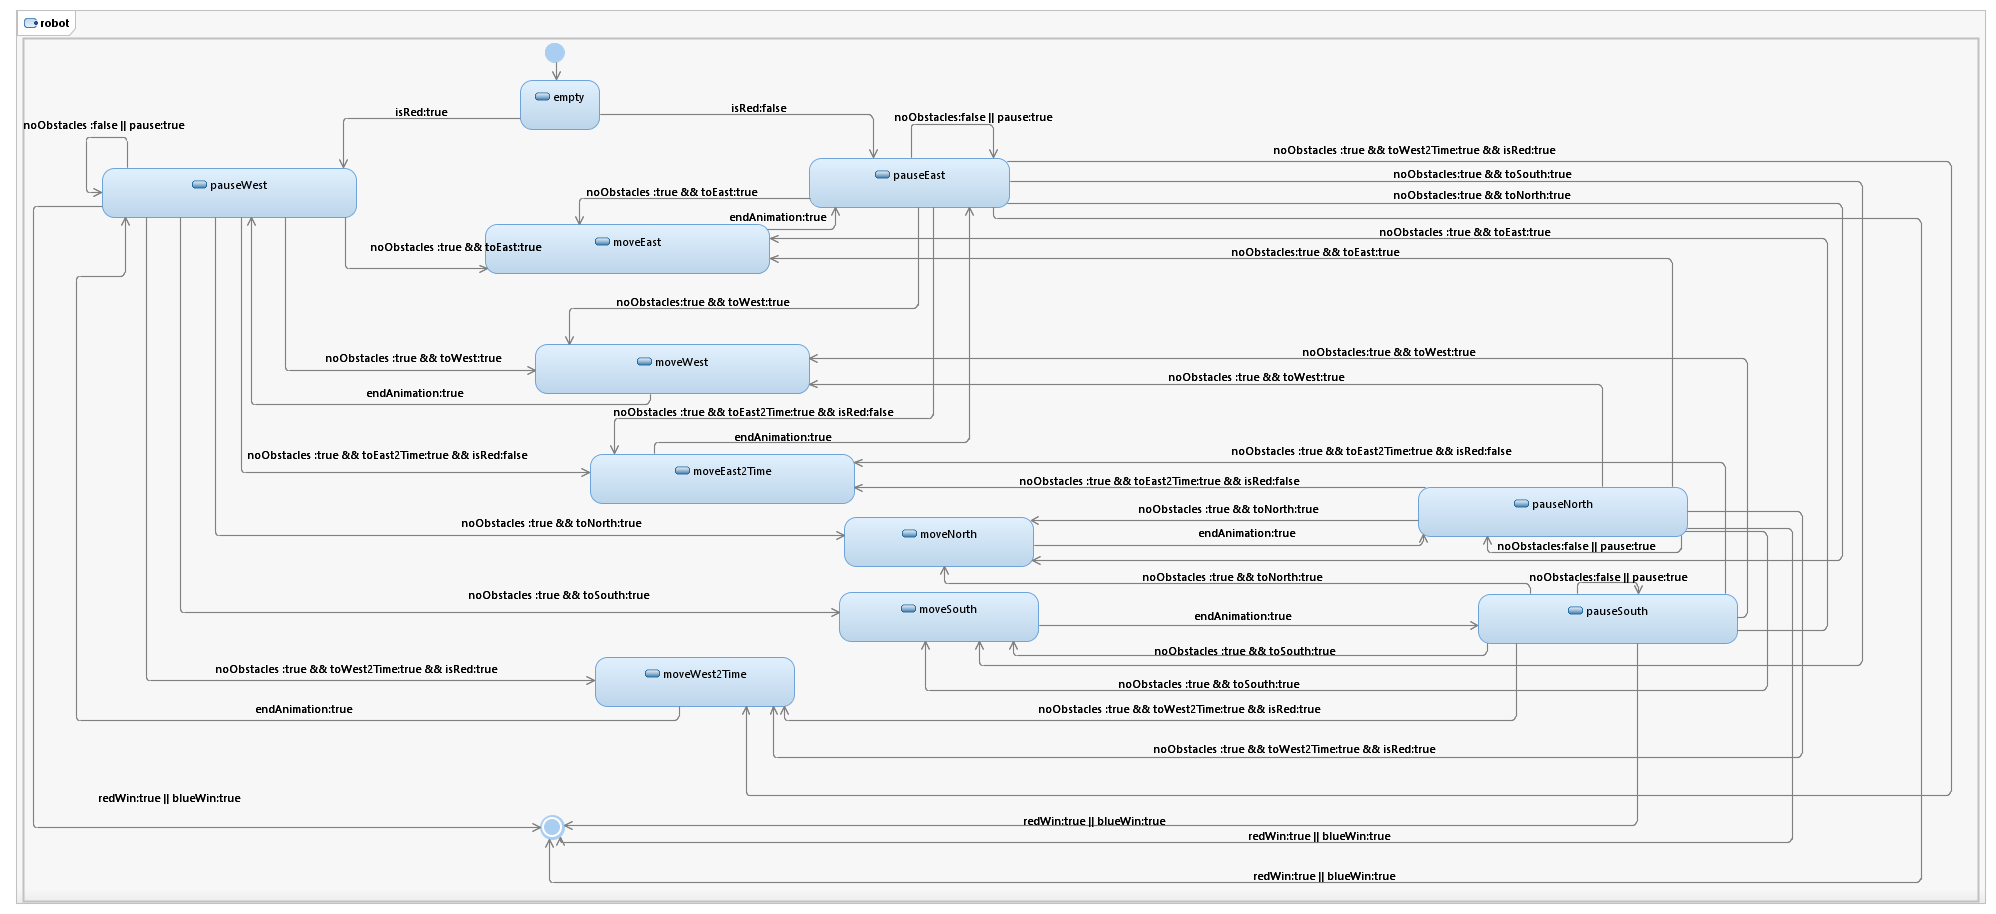
\includegraphics[scale=0.28]{img/state_transition.png}
		\caption{State and transition diagram}
		\label{fig:StateTransition}
	\end{figure}
	
	When the robot moves, if the direction doesn't change, it goes straight forward, but if the direction change, it turns and goes forward at the same time.
	When it doesn't moves, the robot gets a little bit brighter for a second, to show that he's doing an action where it is idle.\\
	On the diagram above, you can see all the different states and conditions of the animations.

\newpage
\section{Protocols of communication}
	\begin{figure}[h]
		\centering
		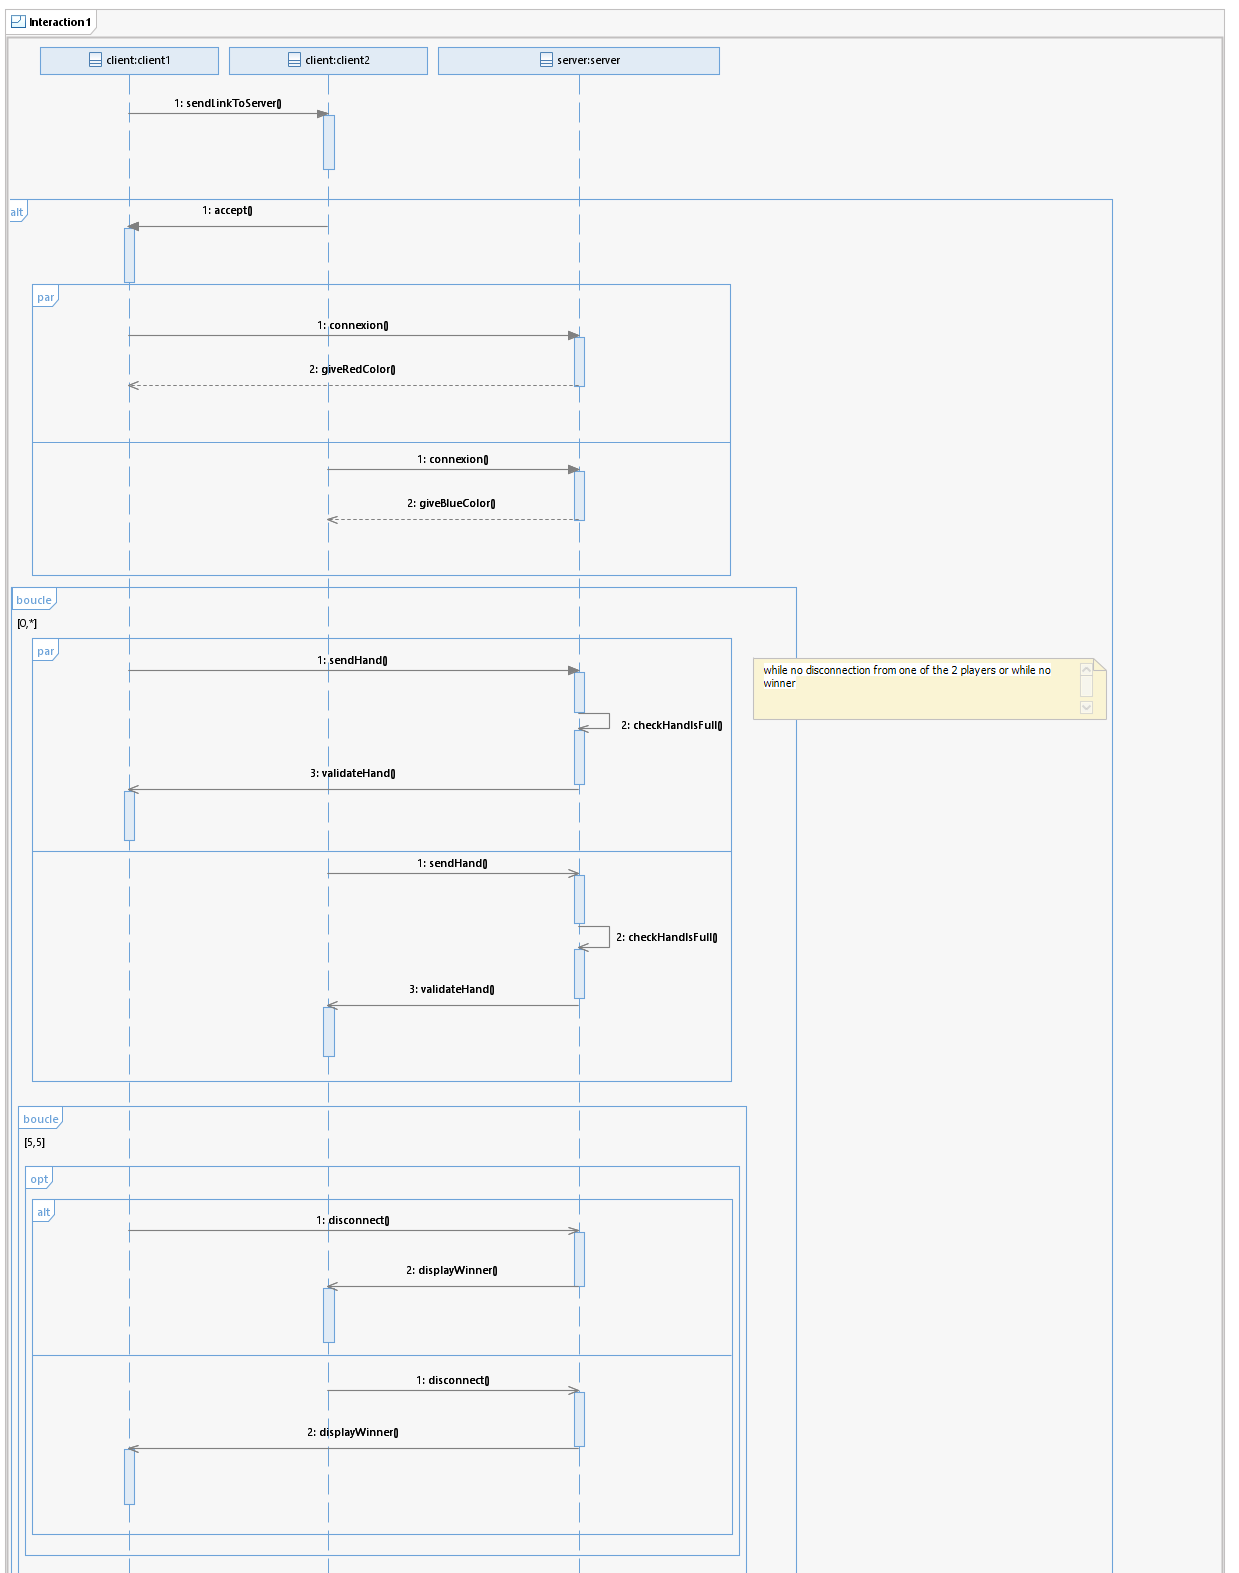
\includegraphics[scale=0.35]{img/sequence1.png}
		\caption{Sequence diagram pt.1}
		\label{fig:Sequence1}
	\end{figure}
	\newpage
	\begin{figure}[h]
		\centering
		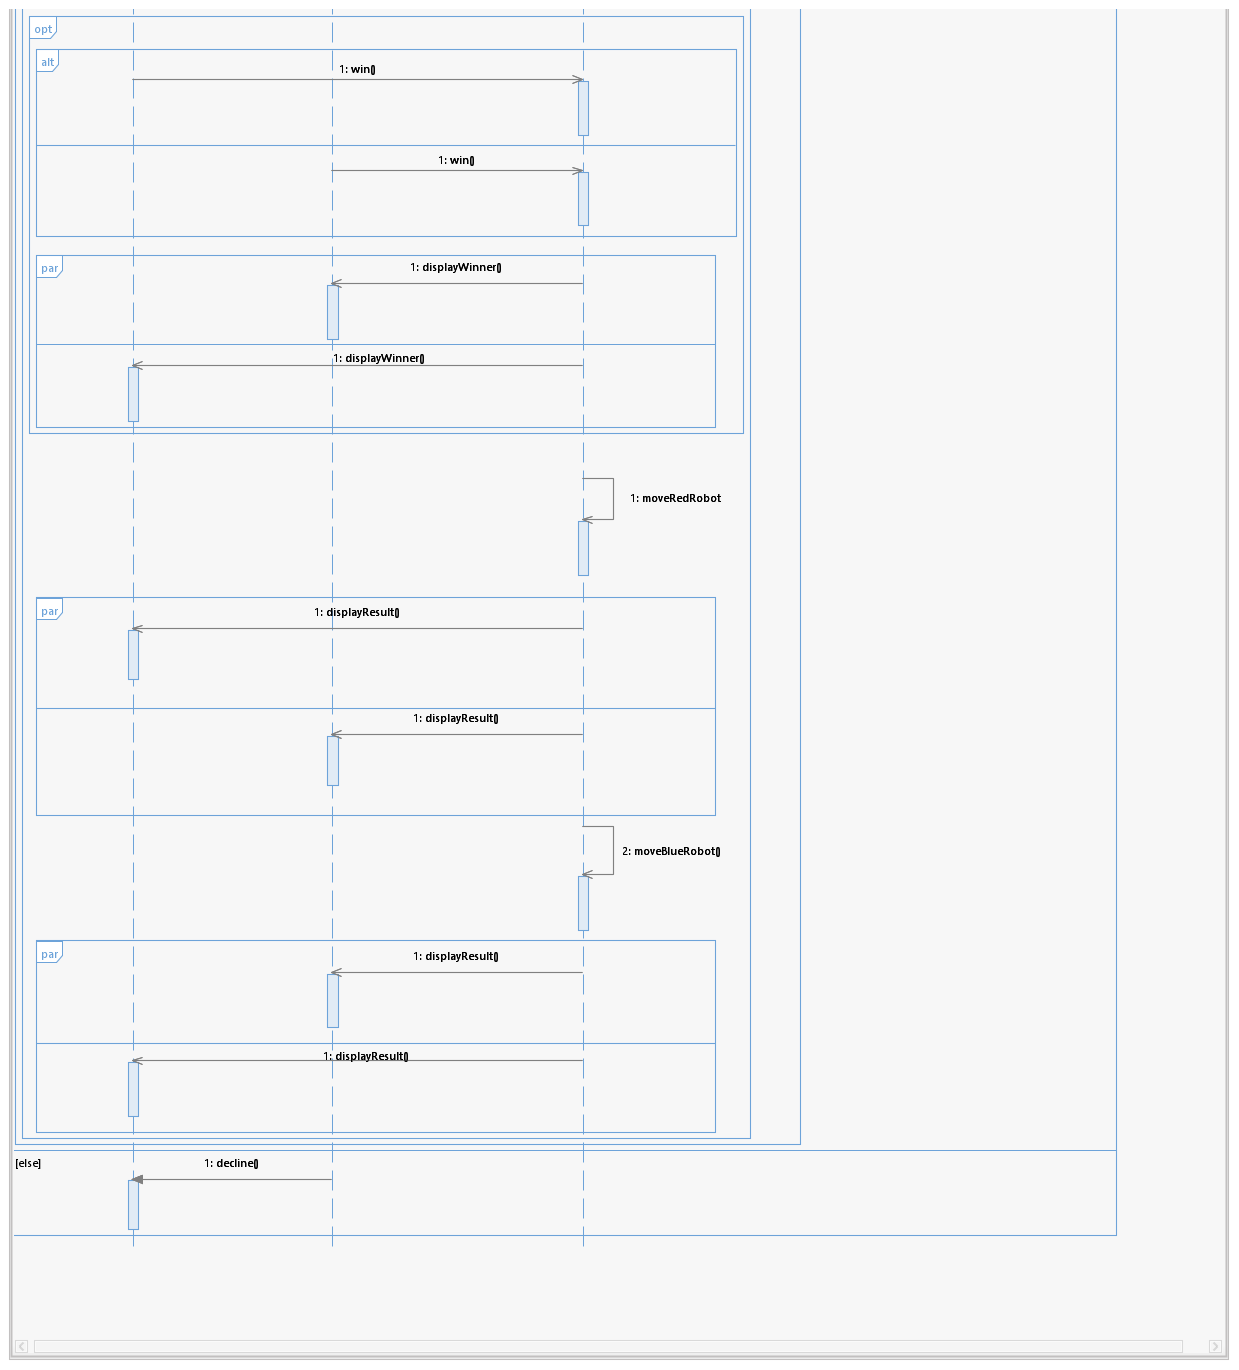
\includegraphics[scale=0.35]{img/sequence2.png}
		\caption{Sequence diagram pt.2}
		\label{fig:Sequence2}
	\end{figure}

\newpage
\section{Work process}
	The work was equally split between us. One of us was in charge of implementing the card selection system and the server modification, when the other was in charge of implementing the progress of the game (the turn, the robot action, \ldots) and making the report. Of course, we also helped each other and worked together when required.\\
	Also, we used GitLab to share our work and manage the different versions of the application.

	\begin{figure}[h]
		\centering
		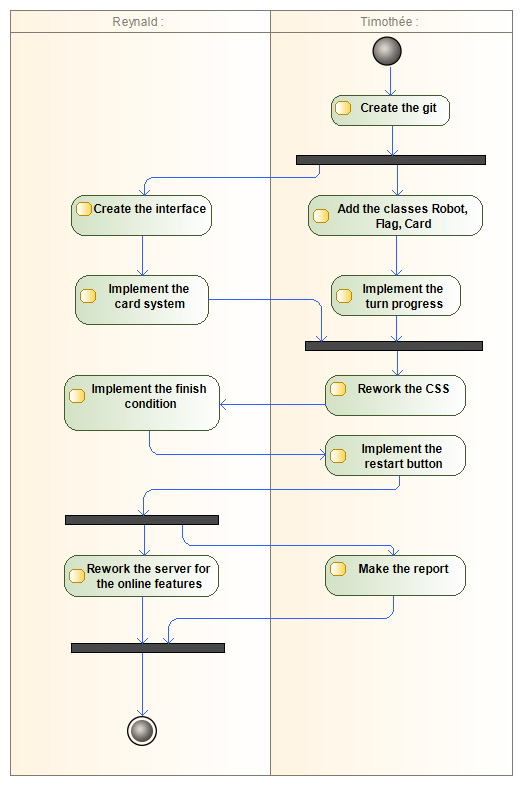
\includegraphics[scale=0.4]{img/activity.png}
		\caption{Activity diagram}
		\label{fig:Activity}
	\end{figure}
	
\newpage
\section{Conclusion}
	We managed to make the local multiplayer game without major difficulties, except the management of the animations that was leading to bugs of position of the HTML elements like the robots or the flags.\\
	The project also extended our practice of Javascript, CSS and HTML, and we are now more at ease with those programming languages and the interactions between them.

\end{document}